% Copyright 2025 Xie Youtian. All rights reserved.
% Confidential - Do not disclose until score of the project is released.
\documentclass{article}
\usepackage{a4}
\usepackage{geometry}
\usepackage{pgf-umlcd}

\usetikzlibrary{arrows.meta}
\geometry{left=1.27cm, right=1.27cm, top=1.27cm, bottom=1.27cm}
\title{Object-oriented Programming \\ Project proposal}
\author{Xie Youtian 2430026233}

\begin{document}
\maketitle
\section{Introduction}
I choose event ticket booking system as my project. 
Below are a kind of business logic of event ticket booking system 
in my recognition and may not be $100\%$ accurate.

In a ticket booking system, users have 3 roles: 
customer, event organizer and administrators. 
We operate with events and tickets.
To simplify the design, we assume that there is no seat arrangement, 
like ACGN conventions or business fairs. 

So, the business logic is clear:
\begin{enumerate}
    \item Customer book, return and change tickets.
    \item Event organizer apply for events and maintain event informations.
    \item System administrator manage users and approve event informations.
\end{enumerate}

\section{Design of OOP Concepts with UML}
Below is a inheritance system of interfaces and classes of users. We use a simple inheritance system to represent the relationship between users, 
and defined what users can do for each type of users.

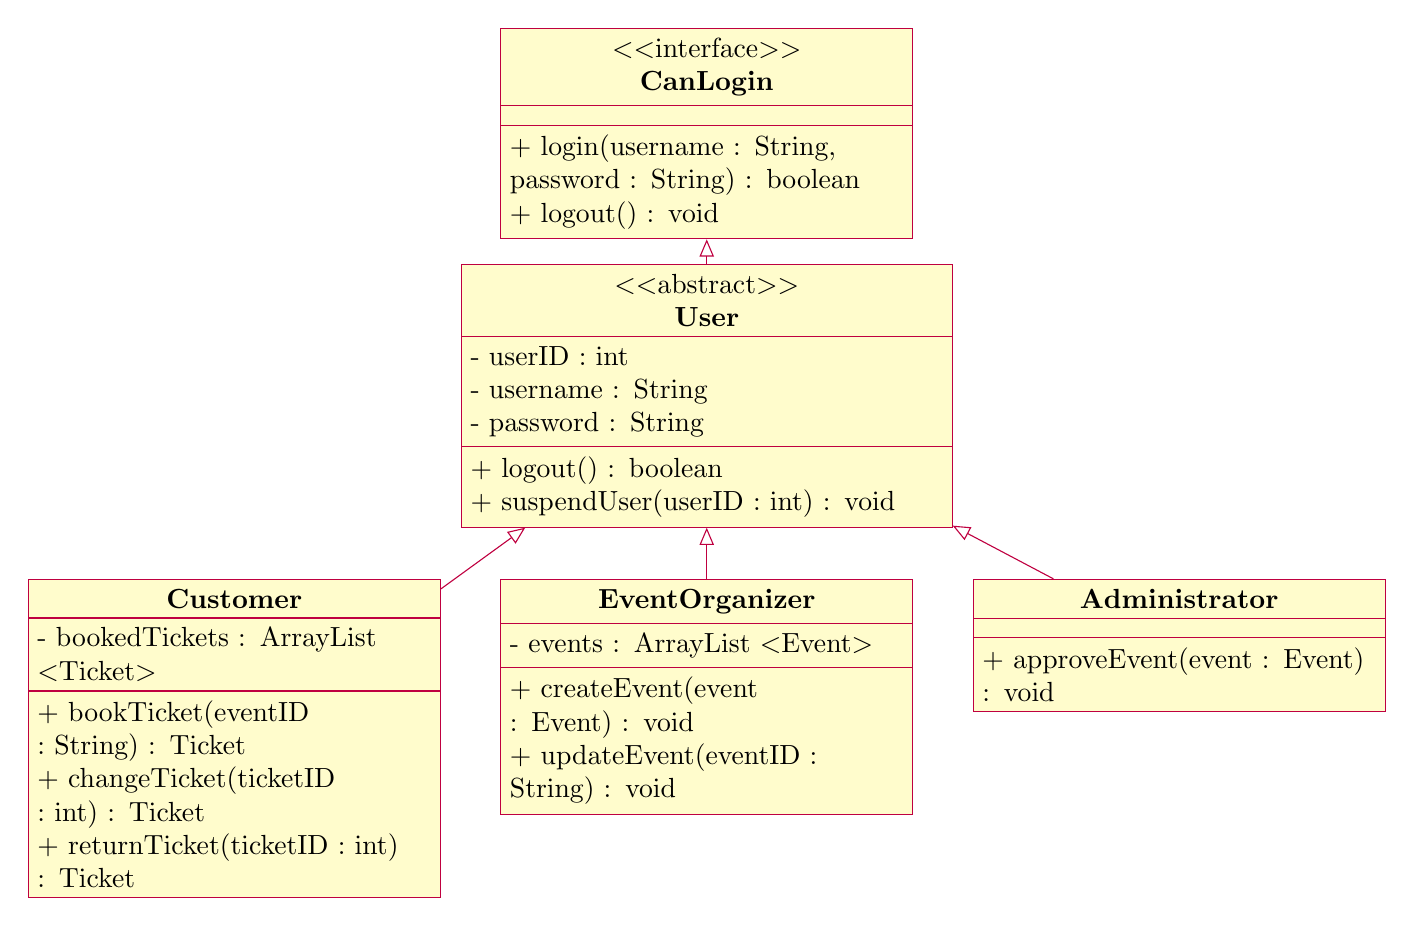
\begin{tikzpicture}
    % 接口定义
    \begin{interface}[text width=5cm]{CanLogin}{0,0}
        \operation{+ login(username : String, password : String) : boolean}
        \operation{+ logout() : void}
    \end{interface}

    % 抽象类
    \begin{abstractclass}[text width=6cm]{User}{0,-3}
        \attribute{- userID : int}
        \attribute{- username : String}
        \attribute{- password : String}
        \operation{+ logout() : boolean}
        \operation{+ suspendUser(userID : int) : void}
        \implement{CanLogin}
    \end{abstractclass}
    
    % 用户继承体系
    \begin{class}[text width=5cm]{Customer}{-6,-7}
        \inherit{User}
        \attribute{- bookedTickets : ArrayList \textless Ticket\textgreater}
        \operation{+ bookTicket(eventID : String) : Ticket}
        \operation{+ changeTicket(ticketID : int) : Ticket}
        \operation{+ returnTicket(ticketID : int) : Ticket}
        % \operation{+ login() : void} % 不允许游客登录
    \end{class}

    \begin{class}[text width=5cm]{EventOrganizer}{0,-7}
        \inherit{User}
        \attribute{- events : ArrayList \textless Event\textgreater}
        \operation{+ createEvent(event : Event) : void}
        \operation{+ updateEvent(eventID : String) : void}
    \end{class}

    \begin{class}[text width=5cm]{Administrator}{6,-7}
        \inherit{User}
        \operation{+ approveEvent(event : Event) : void}
        
    \end{class}
\end{tikzpicture}



\pagebreak
Then let's move to the next step, we need to define the relationship in events. 
First, there is a enumeration type named \textbf{EventStatus} that has 5 values: 
\begin{list}{}{}
    \item \textbf{PLANNING} - Event is planning, but not ready for approval.\\The organizer of this event and administrators can see this event,\\but administrators can't approve it as it is not shown in the waiting list.
    \item \textbf{APPLYING} - Event is applying for approval. When the event organizer updates its information\\it will  go back to \textbf{PLANNING} status.\\Administrators can see this event in the waiting list and decide whether to approve it or not.
    \item \textbf{APPROVED} - Event is approved. All users can see this event, but customers can't book tickets.\\When the event organizer update its information it will go back to \textbf{PLANNING} status.
    \item \textbf{DISAPPROVED} - Event is disapproved, and behaviours are same as \textbf{PLANNING} except on display.
    \item \textbf{AVAILABLE} - Event is available for booking.
    \item \textbf{CANCELLED} - Event is cancelled. All users can see this event, but customers can't book tickets.\\ Other behaviours are same as \textbf{PLANNING}.
\end{list}
 
Below are 3 classes handling event information and ticketing logic, and each \textbf{EventData} is corresponding to a \textbf{Event}.
Implementation will be discussed during the project.

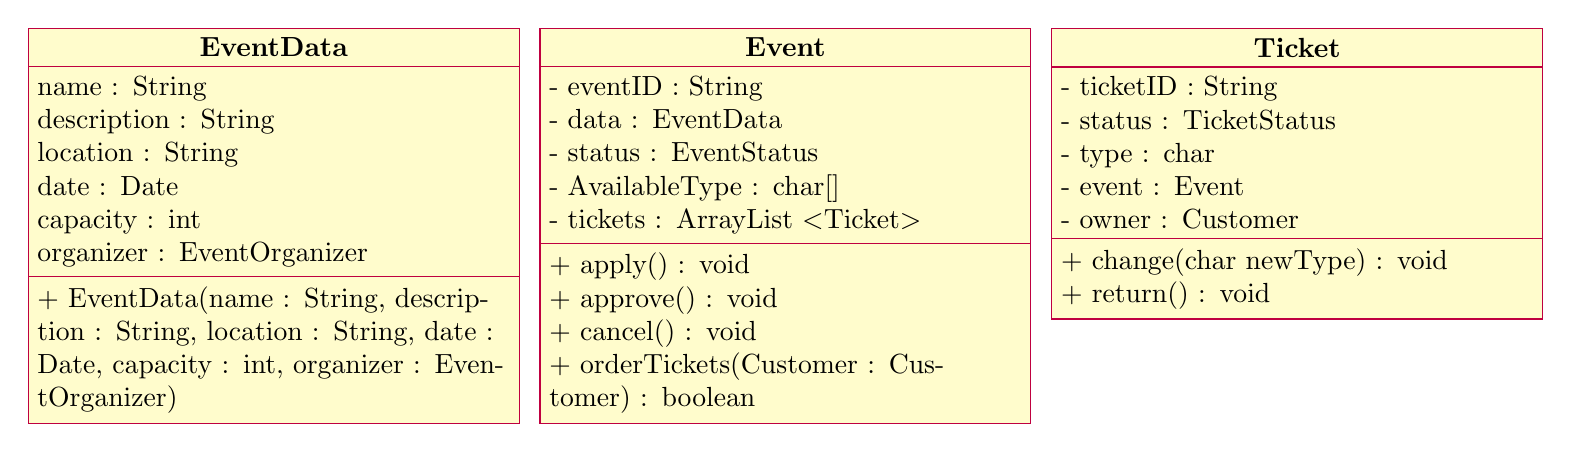
\begin{tikzpicture}

    \begin{class}[text width=6cm]{EventData}{0,0}
        \attribute{name : String}
        \attribute{description : String}
        \attribute{location : String}
        \attribute{date : Date}
        \attribute{capacity : int}
        \attribute{organizer : EventOrganizer}
        \operation{+ EventData(name : String, description : String, location : String, date : Date, capacity : int, organizer : EventOrganizer)}
    \end{class}
    \begin{class}[text width=6cm]{Event}{6.5,0}
        \attribute{- eventID : String}
        \attribute{- data : EventData}
        \attribute{- status : EventStatus}
        \attribute{- AvailableType : char[]}
        \attribute{- tickets : ArrayList \textless Ticket\textgreater}
        \operation{+ apply() : void}
        \operation{+ approve() : void}
        \operation{+ cancel() : void}
        \operation{+ orderTickets(Customer : Customer) : boolean }
    \end{class}
    \begin{class}[text width=6cm]{Ticket}{13,0}
        \attribute{- ticketID : String}
        \attribute{- status : TicketStatus}
        \attribute{- type : char}
        \attribute{- event : Event}
        \attribute{- owner : Customer}
        \operation{+ change(char newType) : void}
        \operation{+ return() : void}
        
    \end{class}
\end{tikzpicture}

Finally, exception handling is also important. Below are expections used in the program and usage of these wxceptions will be determined on demand in actual development.

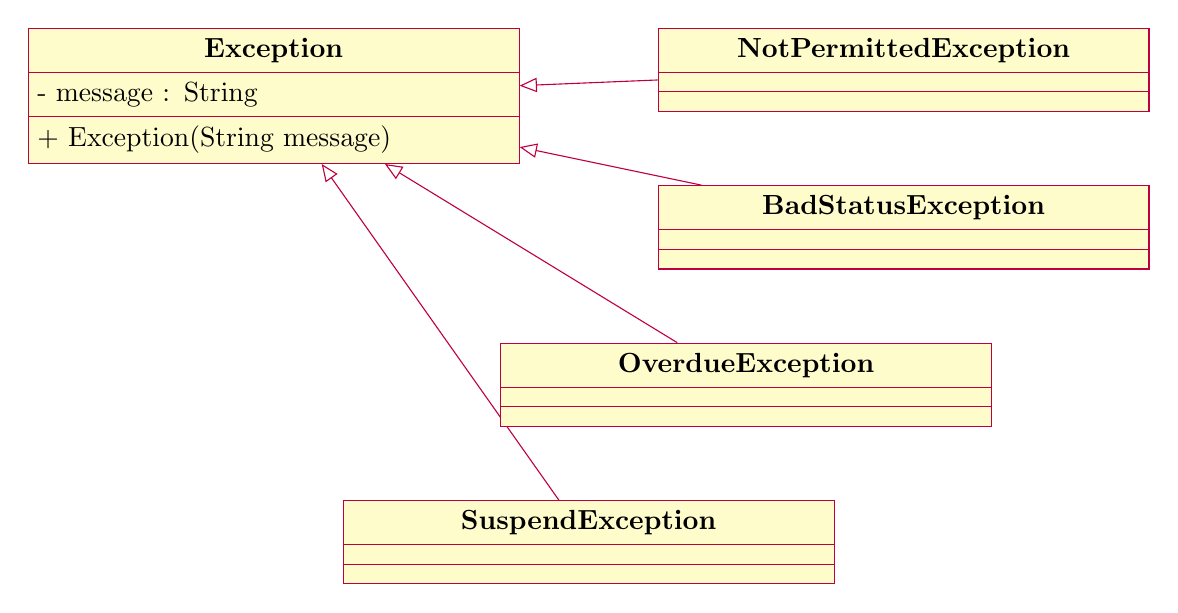
\begin{tikzpicture}
    \begin{class}[text width=6cm]{Exception}{0,0}
        % \inherit{Exception}
        \attribute{- message : String}
        \operation{+ Exception(String message)}
    \end{class}
    \begin{class}[text width=6cm]{NotPermittedException}{8,0}
        \inherit{Exception}
    \end{class}
    \begin{class}[text width=6cm]{BadStatusException}{8,-2}
        \inherit{Exception}
    \end{class}
    \begin{class}[text width=6cm]{OverdueException}{6,-4}
        \inherit{Exception}
    \end{class}
    \begin{class}[text width=6cm]{SuspendException}{4,-6}
        \inherit{Exception}
    \end{class}

\end{tikzpicture}

\pagebreak

\section{Design of user interface}
The prototype of main window is shown in the following picture, which does not represent the final design as Swing library is old and looks ugly while can't be configured easily to look so modern and hygiene.

\includegraphics[width=\textwidth]{Main Window.pdf}
\section{Storage and I/O}
Data will be stored in a SQLite database, with 3 tables: users, tickets and event data. Table name for each table will be named as \verb|tb_user|, \verb|tb_ticket| and \verb|tb_event|.
\\
\hrule

\begin{center}
    This is a prototype of the project, and the actual implementation may be vary from this proposal.\\ 
    All features in this project proposal are subject to change.
    The right to amend the design contained in this proposal, \\containing but not limited to OOP design, UI/UX design amd data storage is reserved.

    \copyright 2025 Xie Youtian. All rights reserved.
\end{center}
\end{document}